\documentclass{article} % say
\usepackage{tikz}
\begin{document}
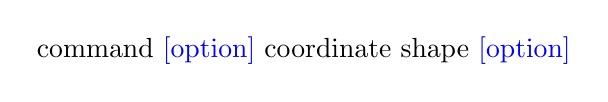
\begin{tikzpicture}
  %% [scale=3,
  %%   line cap=round,
  %%   % Styles
  %%   axes/.style=,
  %%   important line/.style={very thick},
  %%   information text/.style={rounded corners, fill=red!10, inner sep=1ex}]

  %% %% Colors
  %% \colorlet{anglecolor}{green!50!black}
  %% \colorlet{sincolor}{red}
  %% \colorlet{tancolor}{orange!80!black}
  %% \colorlet{coscolor}{blue}

  %% %% The graphic
  %% \draw[help lines,step=.5cm] (-1.4,-1.4) grid (1.4,1.4); 

  %% \draw (0,0) circle [radius=1cm];

  %% \begin{scope}[axes]
  %%   \draw[->] (-1.5,0) -- (1.5,0) node[right] {$x$} coordinate(x axis); % axis
  %%   \draw[->] (0,-1.5) -- (0,1.5) node[right] {$x$} coordinate(y axis); % axis

  %%   \foreach \x/\xtext in {-1,-0.5/-\frac{1}{2},1} \draw (\x cm,-1pt) -- (\x cm,1pt) node[anchor=north,fill=white] {$\xtext$};
  %%   \foreach \y/\ytext in {-1,-0.5/-\frac{1}{2},0.5/\frac{1}{2},1}  \draw (-1pt,\y cm) -- (1pt,\y cm) node[anchor=east,fill=white] {$\ytext$};
  %% \end{scope}

  %% \filldraw[fill=green!20,draw=anglecolor] (0,0) -- (3mm,0mm)
  %% arc [start angle=0, end angle=30, radius=3mm] -- cycle; % angle

  %% %% math line
  %% \draw[important line,sincolor] (30:1cm) -- node[left=1pt,fill=white] {$\sin \alpha$} +(0,-0.5); % sin
  %% \draw[important line,coscolor] (30:1cm) ++(0,-0.5) -- node[below=2pt,fill=white] {$\cos \alpha$} (0,0); % cos
  %% \draw[very thick,orange] (1,0) -- node[right=1pt,fill=white]
  %%      {$\displaystyle \tan \alpha \color{black} =\frac{{\color{red}\sin \alpha}}{\color{blue}\cos \alpha}$} (1,{tan(30)});                        % tan

  %%      \draw (0,0) -- (1,{tan(30)});

  %% \draw[xshift=1.85cm]
  %% node[right,text width=6cm,information text] {
  %%   The {\color{anglecolor} angle $\alpha$} is $30^\circ$ in the
  %%   example ($\pi/6$ in radians). The {\color{sincolor}sine of
  %%     $\alpha$}, which is the height of the red line, is
  %%   \[
  %%     {\color{sincolor} \sin \alpha} = 1/2. \]
  %%     By the Theorem of Pythagoras ...
  %% };

  \colorlet{optioncolor}{blue}
  
  \draw node{ command {\color{optioncolor}[option]} coordinate shape {\color{optioncolor}[option]}};



        
\end{tikzpicture}



\end{document}
